\documentclass[class=minimal, border = 0pt, crop]{standalone}
\usepackage{pgf}
\usepackage{tikz}
\usepackage[utf8]{inputenc}
\usetikzlibrary{arrows,automata,shapes,calc, backgrounds}
\usetikzlibrary{positioning}
\pagestyle{empty}
\tikzset{
    state/.style={
           rectangle,
           rounded corners,
           draw=black, very thick,
           minimum height=2em,
           inner sep=5pt,
           text centered,
           },
    pil/.style={
           ->,
           thick,
           shorten <=4pt,
           shorten >=4pt,}
}
\begin{document}
\centering
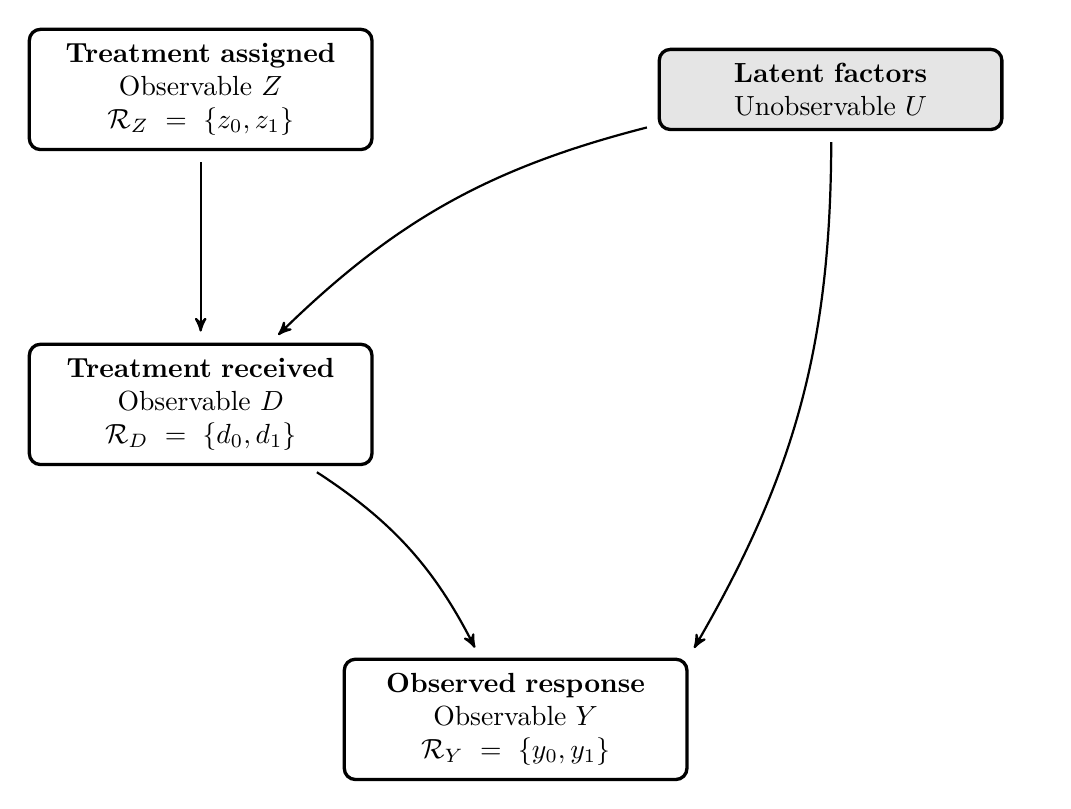
\begin{tikzpicture}[->,>=stealth']
% BASIC MODEL
% Position of Treatment assigned (ASSIGN)
\node[state, text width = 4cm] (ASSIGN)
{
\textbf{Treatment assigned}\\
Observable $Z$\\
$\mathcal{R}_Z=\lbrace z_0,z_1\rbrace$\\
};
% Position of Treatment received (RECEIVE)
\node[state,
text width = 4cm,
below of = ASSIGN,
node distance = 4cm] (RECEIVE)
{\textbf{Treatment received}\\
Observable $D$\\
$\mathcal{R}_D=\lbrace d_0,d_1\rbrace$\\
};
% Position of Observed response (OUTCOME)
\node[state,
text width = 4cm,
below of = RECEIVE,
node distance = 4cm,
xshift = 4cm] (OUTCOME)
{\textbf{Observed response}\\
Observable $Y$\\
$\mathcal{R}_Y=\lbrace y_0,y_1\rbrace$\\
};
% Position of Latent factors (LATENT)
\node[state,
text width = 4cm,
right of = ASSIGN,
node distance = 8cm,
fill = gray!20,
label = right:\phantom{$T$}] (LATENT)
{\textbf{Latent factors}\\
Unobservable $U$\\
};
% Draw lines on graph
\path (LATENT) edge[pil, bend left = 15] (OUTCOME.north east);
\path (LATENT) edge[pil, bend right = 15] (RECEIVE);
\path (ASSIGN) edge[pil] (RECEIVE);
\path (RECEIVE) edge[pil, bend left = 15] (OUTCOME);
\end{tikzpicture}
\end{document}